% Options for packages loaded elsewhere
\PassOptionsToPackage{unicode}{hyperref}
\PassOptionsToPackage{hyphens}{url}
\documentclass[
  11pt,
]{article}
\usepackage{xcolor}
\usepackage[margin=1in]{geometry}
\usepackage{amsmath,amssymb}
\setcounter{secnumdepth}{-\maxdimen} % remove section numbering
\usepackage{iftex}
\ifPDFTeX
  \usepackage[T1]{fontenc}
  \usepackage[utf8]{inputenc}
  \usepackage{textcomp} % provide euro and other symbols
\else % if luatex or xetex
  \usepackage{unicode-math} % this also loads fontspec
  \defaultfontfeatures{Scale=MatchLowercase}
  \defaultfontfeatures[\rmfamily]{Ligatures=TeX,Scale=1}
\fi
\usepackage{lmodern}
\ifPDFTeX\else
  % xetex/luatex font selection
\fi
% Use upquote if available, for straight quotes in verbatim environments
\IfFileExists{upquote.sty}{\usepackage{upquote}}{}
\IfFileExists{microtype.sty}{% use microtype if available
  \usepackage[]{microtype}
  \UseMicrotypeSet[protrusion]{basicmath} % disable protrusion for tt fonts
}{}
\makeatletter
\@ifundefined{KOMAClassName}{% if non-KOMA class
  \IfFileExists{parskip.sty}{%
    \usepackage{parskip}
  }{% else
    \setlength{\parindent}{0pt}
    \setlength{\parskip}{6pt plus 2pt minus 1pt}}
}{% if KOMA class
  \KOMAoptions{parskip=half}}
\makeatother
\usepackage{longtable,booktabs,array}
\usepackage{calc} % for calculating minipage widths
% Correct order of tables after \paragraph or \subparagraph
\usepackage{etoolbox}
\makeatletter
\patchcmd\longtable{\par}{\if@noskipsec\mbox{}\fi\par}{}{}
\makeatother
% Allow footnotes in longtable head/foot
\IfFileExists{footnotehyper.sty}{\usepackage{footnotehyper}}{\usepackage{footnote}}
\makesavenoteenv{longtable}
\usepackage{graphicx}
\makeatletter
\newsavebox\pandoc@box
\newcommand*\pandocbounded[1]{% scales image to fit in text height/width
  \sbox\pandoc@box{#1}%
  \Gscale@div\@tempa{\textheight}{\dimexpr\ht\pandoc@box+\dp\pandoc@box\relax}%
  \Gscale@div\@tempb{\linewidth}{\wd\pandoc@box}%
  \ifdim\@tempb\p@<\@tempa\p@\let\@tempa\@tempb\fi% select the smaller of both
  \ifdim\@tempa\p@<\p@\scalebox{\@tempa}{\usebox\pandoc@box}%
  \else\usebox{\pandoc@box}%
  \fi%
}
% Set default figure placement to htbp
\def\fps@figure{htbp}
\makeatother
% definitions for citeproc citations
\NewDocumentCommand\citeproctext{}{}
\NewDocumentCommand\citeproc{mm}{%
  \begingroup\def\citeproctext{#2}\cite{#1}\endgroup}
\makeatletter
 % allow citations to break across lines
 \let\@cite@ofmt\@firstofone
 % avoid brackets around text for \cite:
 \def\@biblabel#1{}
 \def\@cite#1#2{{#1\if@tempswa , #2\fi}}
\makeatother
\newlength{\cslhangindent}
\setlength{\cslhangindent}{1.5em}
\newlength{\csllabelwidth}
\setlength{\csllabelwidth}{3em}
\newenvironment{CSLReferences}[2] % #1 hanging-indent, #2 entry-spacing
 {\begin{list}{}{%
  \setlength{\itemindent}{0pt}
  \setlength{\leftmargin}{0pt}
  \setlength{\parsep}{0pt}
  % turn on hanging indent if param 1 is 1
  \ifodd #1
   \setlength{\leftmargin}{\cslhangindent}
   \setlength{\itemindent}{-1\cslhangindent}
  \fi
  % set entry spacing
  \setlength{\itemsep}{#2\baselineskip}}}
 {\end{list}}
\usepackage{calc}
\newcommand{\CSLBlock}[1]{\hfill\break\parbox[t]{\linewidth}{\strut\ignorespaces#1\strut}}
\newcommand{\CSLLeftMargin}[1]{\parbox[t]{\csllabelwidth}{\strut#1\strut}}
\newcommand{\CSLRightInline}[1]{\parbox[t]{\linewidth - \csllabelwidth}{\strut#1\strut}}
\newcommand{\CSLIndent}[1]{\hspace{\cslhangindent}#1}
\setlength{\emergencystretch}{3em} % prevent overfull lines
\providecommand{\tightlist}{%
  \setlength{\itemsep}{0pt}\setlength{\parskip}{0pt}}
\usepackage{graphicx}
\graphicspath{{./figures/}}
\usepackage{hyperref}
\hypersetup{colorlinks=true,linkcolor=blue,urlcolor=blue,citecolor=blue}
\usepackage{parskip}
\setlength{\parskip}{0.25\baselineskip}
\renewcommand{\bfdefault}{b}
\renewcommand{\bfseries}{\mdseries\bfseries}
\usepackage{bookmark}
\IfFileExists{xurl.sty}{\usepackage{xurl}}{} % add URL line breaks if available
\urlstyle{same}
\hypersetup{
  pdftitle={Normative Executive System (NES): A Proof-of-Concept Computational Testbed for Identifiable Normative Influence},
  pdfauthor={Jesse Wright},
  hidelinks,
  pdfcreator={LaTeX via pandoc}}

\title{Normative Executive System (NES): A Proof-of-Concept
Computational Testbed for Identifiable Normative Influence}
\author{Jesse Wright}
\date{May 8, 2025}

\begin{document}
\maketitle
\begin{abstract}
We propose that normative influence in human decision-making is
computationally primitive---not emergent from utility maximization,
emotional response, or social learning---but a fundamental architectural
component of moral cognition. To test this theoretical claim, we
introduce the Normative Executive System (NES), extending the Drift
Diffusion Model with an explicit norm weight parameter (\(w_n\)) that
modulates decision dynamics independently of utility-based signals. Our
empirical test employs Simulation-Based Calibration across multiple
inference methods (ABC-SMC and Neural Posterior Estimation), revealing
the key finding that \(w_n\) is statistically identifiable from
behavioral data, suggesting normative influence leaves distinct
computational signatures unexplained by existing models. A critical
result emerged from standard hierarchical DDMs, which---even when
enhanced with regression over conflict conditions---systematically
failed to recover \(w_n\) from NES-generated data, highlighting
representational limits under NES-like task conditions. These results
provide the first direct computational evidence that moral
decision-making benefits from explicit normative representation,
establishing a formal dissociation between normative and general
value-based choice models. The findings suggest that normative
self-governance is not merely an emergent byproduct, but a measurable
and computationally distinct faculty, offering new pathways for
understanding moral cognition.

\emph{Keywords:} Normative Executive System; Moral Cognition; Drift
Diffusion Model; Simulation-Based Inference; Norm Weight; Decision
Neuroscience
\end{abstract}

\newpage

\section{1. Norm-Governed Decisions: A Computational
Puzzle}\label{norm-governed-decisions-a-computational-puzzle}

People routinely make norm-consistent choices even when payoff, emotion,
and cognitive control all favor defection. We stop at red lights on
empty roads, keep unenforceable promises, and help strangers at our own
expense. These behaviors persist even when material incentives or
learned associations would push us the other way---suggesting an
internal mechanism that cannot be reduced to reward, affect, or generic
control.

Most formal models of decision-making subsume norms under emergent
processes within general-purpose architectures:

\begin{itemize}
\tightlist
\item
  \textbf{Utility models} treat norms as high-value preferences\\
\item
  \textbf{Learning theories} invoke conditioned associations via social
  feedback\\
\item
  \textbf{Dual-process accounts} emphasize emotional inhibition or
  deliberative override\\
\item
  \textbf{Conflict-monitoring frameworks} cast restraint as
  domain-general control
\end{itemize}

Under these views, norm-adherence arises ``for free'' as a byproduct of
utility maximization, social learning, or inhibitory control. Yet many
moral choices strike us as uncued, unsupervised, and unmotivated by
self-interest---prompting a different question:

\begin{quote}
\emph{Could normative influence itself be a primitive component of the
decision architecture?}
\end{quote}

To explore this, we introduce the \textbf{Normative Executive System
(NES)}, a minimal extension of the Drift Diffusion Model (DDM) that
encodes an explicit \textbf{norm weight} (\(w_n\)) alongside standard
salience and threshold parameters. By embedding \(w_n\) directly into
the drift equation, NES operationalizes the hypothesis that norms exert
a distinct, recoverable pull on evidence accumulation---rather than
emerging from other model dimensions.

Recent reviews highlight a lack of empirical tests for whether explicit
normative representations are necessary to capture moral behavior
(\citeproc{ref-bello2023computationalapproachesto}{Bello \& Malle,
2023}; \citeproc{ref-cushman2015moralconstraints}{Cushman, 2015}). NES
targets this gap by using \textbf{Simulation-Based Calibration} (ABC-SMC
and Neural Posterior Estimation) to ask three questions:

\begin{enumerate}
\def\labelenumi{\arabic{enumi}.}
\tightlist
\item
  \textbf{Identifiability:} Is \(w_n\) statistically recoverable from
  simulated behavior?\\
\item
  \textbf{Distinctiveness:} Does NES generate decision patterns that
  standard DDMs cannot reproduce by parameter tuning alone?\\
\item
  \textbf{Structural Mismatch:} Do fortified hierarchical DDMs
  systematically fail to recover \(w_n\) from NES-generated data?
\end{enumerate}

By shifting the debate from philosophical intuition to statistical
identifiability and predictive utility, NES provides a formal, testable
framework for investigating whether normative self-governance is a
measurable, architecturally distinct faculty in human decision-making.

\subsection{1.1 Related Work}\label{related-work}

NES builds on a rich tradition of cognitive modeling, including the
conflict monitoring framework
(\citeproc{ref-Botvinick2001ConflictMonitoring}{Botvinick et al.,
2001}), dual-process theories of moral judgment
(\citeproc{ref-Greene2001fMRI}{Greene et al., 2001}), and attribute-wise
value integration models (\citeproc{ref-Hare2009SelfControl}{Hare et
al., 2009}). However, these models either lack explicit norm
representations or do not validate the identifiability of such
constructs from behavior. NES proposes a principled extension of the
Drift Diffusion Model that treats norm influence as an independent
signal---recoverable and separable from salience or utility.

\section{2. The Normative Executive System: Formalizing Primitive Moral
Architecture}\label{the-normative-executive-system-formalizing-primitive-moral-architecture}

\subsection{2.1 Core Architectural
Principle}\label{core-architectural-principle}

The \textbf{Normative Executive System (NES)} extends the classic Drift
Diffusion Model by adding a dedicated \textbf{norm weight} (\(w_n\))
alongside the standard salience weight (\(w_s\)). The drift rate is
defined as

\[
v = w_s\,(1 - \lambda)\;-\;w_n\,\lambda
\]

where \(\lambda\in[0,1]\) indexes conflict between stimulus salience and
internalized norms. Setting \(w_n\) apart as its own parameter creates
an \textbf{oppositional architecture} in which norms exert a direct,
quantifiable pull on evidence accumulation rather than being folded into
existing utility or control signals.

\subsection{2.2 Why This Tests Computational
Primitiveness}\label{why-this-tests-computational-primitiveness}

This simple formulation makes three critical tests possible:

\begin{enumerate}
\def\labelenumi{\arabic{enumi}.}
\tightlist
\item
  \textbf{Oppositional Architecture:} By pitting \(w_s\) vs.~\(w_n\) in
  direct competition, we force the model to resolve norm--salience
  conflict explicitly.\\
\item
  \textbf{Parameter Independence:} Because \(w_n\) is not a transform of
  other variables, its recoverability signals a true architectural
  primitive.\\
\item
  \textbf{Graded Conflict:} Continuous variation in \(\lambda\) lets us
  probe whether the model responds systematically across low to high
  conflict---a hallmark of dedicated processing.
\end{enumerate}

\subsection{2.3 Architectural
Predictions}\label{architectural-predictions}

NES yields three testable predictions that distinguish it from
emergentist accounts:

\begin{enumerate}
\def\labelenumi{\arabic{enumi}.}
\tightlist
\item
  \textbf{Behavioral Signatures:} Unique reaction-time and error-rate
  patterns (e.g., non-monotonic RT under high \(\lambda\), systematic
  response suppression) that standard DDMs cannot mimic.\\
\item
  \textbf{Statistical Identifiability:} The norm weight \(w_n\) should
  be recoverable from choice/RT data with minimal ambiguity.\\
\item
  \textbf{Architectural Irreducibility:} Models lacking an explicit
  \(w_n\) should systematically fail to capture key norm-driven dynamics
  when fit to NES-generated data.
\end{enumerate}

\subsection{2.4 Simulation \& Inference
Overview}\label{simulation-inference-overview}

To evaluate these predictions, we implemented NES in a standard DDM
framework (see Supplement A for full details). Briefly:

\begin{itemize}
\tightlist
\item
  \textbf{Task:} A parametric ``Stroop-like'' conflict paradigm with
  five \(\lambda\) levels and moderate trial counts to test
  identifiability under realistic session lengths.\\
\item
  \textbf{Simulation:} Euler--Maruyama integration generates choice/RT
  data under known \((w_s,w_n,\lambda)\) settings.\\
\item
  \textbf{Inference:} We apply both \textbf{ABC-SMC} and \textbf{Neural
  Posterior Estimation (NPE)} to assess recovery of \(w_n\) (Supplement
  B).\\
\item
  \textbf{Benchmark:} A fortified hierarchical HDDM model---with
  per-condition drift regressors---tests whether standard approaches can
  indirectly recover \(w_n\).
\end{itemize}

\subsection{2.5 Key Validation Steps}\label{key-validation-steps}

\begin{enumerate}
\def\labelenumi{\arabic{enumi}.}
\tightlist
\item
  \textbf{Identifiability:} SBC rank‐histograms for both ABC-SMC and NPE
  should approximate uniformity, indicating well-calibrated recovery of
  \(w_n\).\\
\item
  \textbf{HDDM Failure:} If HDDM's drift regressions produce biased or
  uncalibrated \(w_n\) estimates, this confirms an architectural
  mismatch.\\
\item
  \textbf{Behavioral Signatures:} Simulated RT/error curves under
  varying \(w_n\) should reveal patterns (e.g., conflict-conditioned
  suppression) unique to NES.
\end{enumerate}

By keeping the core drift equation and predictions
front-and-center---and delegating algorithmic details, parameter
settings, and summary‐statistic choices to the Supplement---this section
emphasizes NES's conceptual contribution while reserving technical depth
for specialist readers.

\subsection{\texorpdfstring{2.6 HDDM Recovery of
\(w_n\)}{2.6 HDDM Recovery of w\_n}}\label{hddm-recovery-of-w_n}

\subsubsection{2.5.1 Pipeline Validation (Standard DDM
Data)}\label{pipeline-validation-standard-ddm-data}

Before analyzing NES data, we first validated our HDDM implementation on
standard DDM-simulated data. Five synthetic subjects each completed 3000
trials generated with true values of \(a = 1.5\), \(v = 0.5\), and
\(t_0 = 0.2\). The recovered posterior distributions are shown in Figure
1.

All parameters were accurately recovered, with posterior mass
concentrated around ground truth values and all estimates falling within
5\% of their respective true values. This confirms that the HDDM stack
is functioning as expected under its own assumptions.

\begin{figure}
\centering
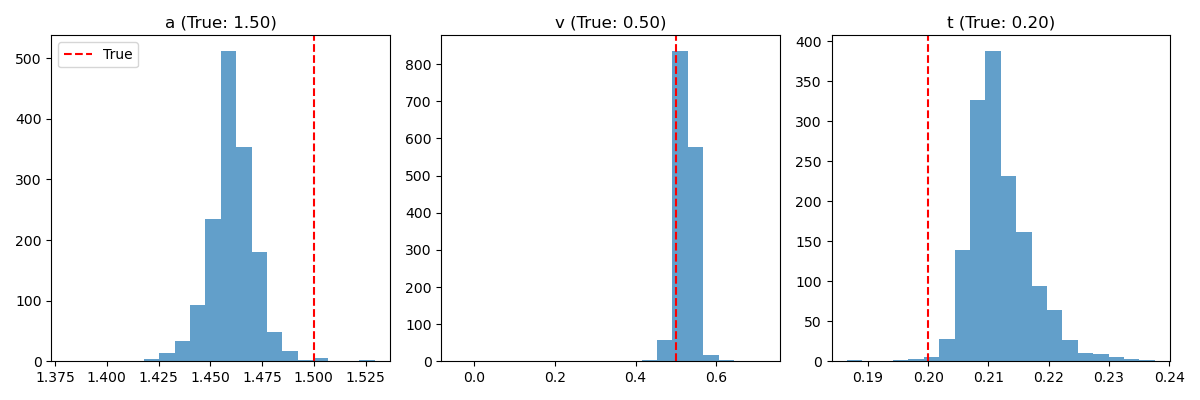
\includegraphics[width=0.9\linewidth,height=\textheight,keepaspectratio]{figures/hddm_sanity_check.png}
\caption{Posterior distributions for \(a\), \(v\), and \(t_0\) recovered
by HDDM on standard DDM-simulated data.}\label{fig:hddm_sanity}
\end{figure}

\subsubsection{2.5.2 Fortified HDDM on NES
Data}\label{fortified-hddm-on-nes-data}

We next tested whether HDDM could indirectly recover \(w_n\) when
applied to NES-simulated data. To give HDDM every possible advantage, we
implemented a fortified hierarchical model with per-condition drift
regressors. The setup was as follows:

\begin{itemize}
\tightlist
\item
  \textbf{True values}: \(w_n \sim \mathrm{Uniform}(0.1, 2.0)\)\\
\item
  \textbf{Simulated data}: NES-DDM with 5 subjects × 1000 trials; 5
  \(\lambda\) levels\\
\item
  \textbf{Fit model}: HDDM with group-level estimates of \(a\), \(t_0\),
  and \(v(\lambda)\)\\
\item
  \textbf{Derived \(w_n\)}: slope from regression of drift rates on
  conflict\\
\item
  \textbf{SBC}: ranks of inferred \(w_n\) vs.~ground truth
\end{itemize}

The results were unambiguous: - \textbf{Parameter recovery} was poor:
Pearson \(r = 0.29\)--0.62, \(R^2 = 0.05\)--0.38\\
- \textbf{Systematic bias} was observed (e.g., \(v_{0.5}\) bias =
−0.48)\\
- \textbf{Coverage within ±0.1} was only 21\%--35\%\\
- \textbf{SBC ranks} were maxed out (rank = 1000), indicating severe
overconfidence and miscalibration

\begin{figure}
\centering
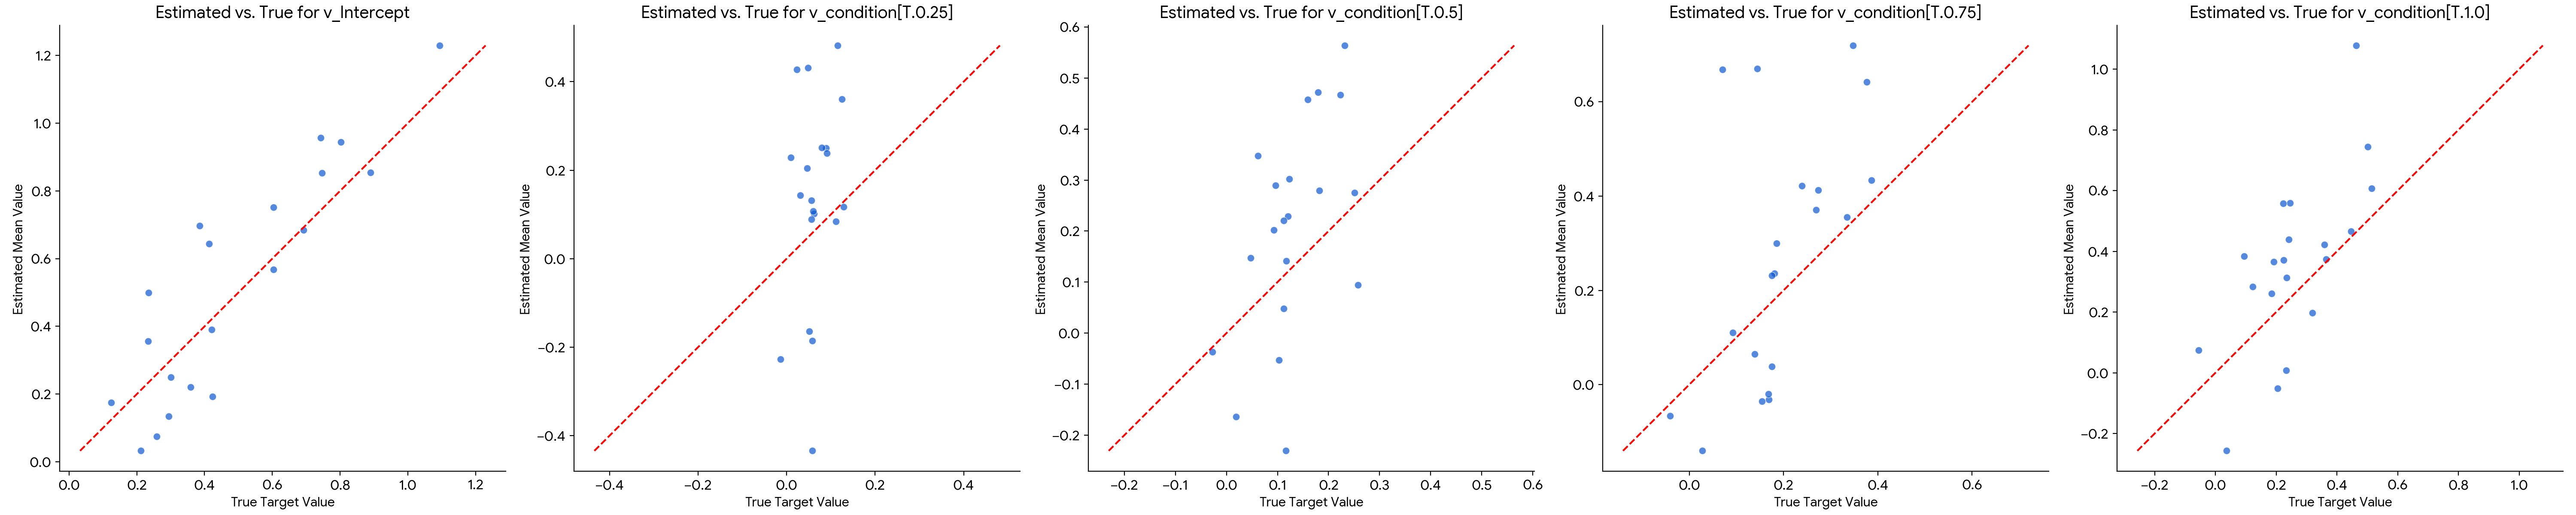
\includegraphics[width=0.9\linewidth,height=\textheight,keepaspectratio]{figures/fortified_hddm_chart.png}
\caption{Comparison of true vs.~estimated drift rates across conflict
levels from HDDM applied to NES-simulated data. Each point represents
one SBC iteration (subject-averaged group estimate). Systematic
deviation from the identity line indicates consistent misrecovery of
drift rate dynamics due to architectural
mismatch.}\label{fig:fortified_chart}
\end{figure}

\begin{figure}
\centering
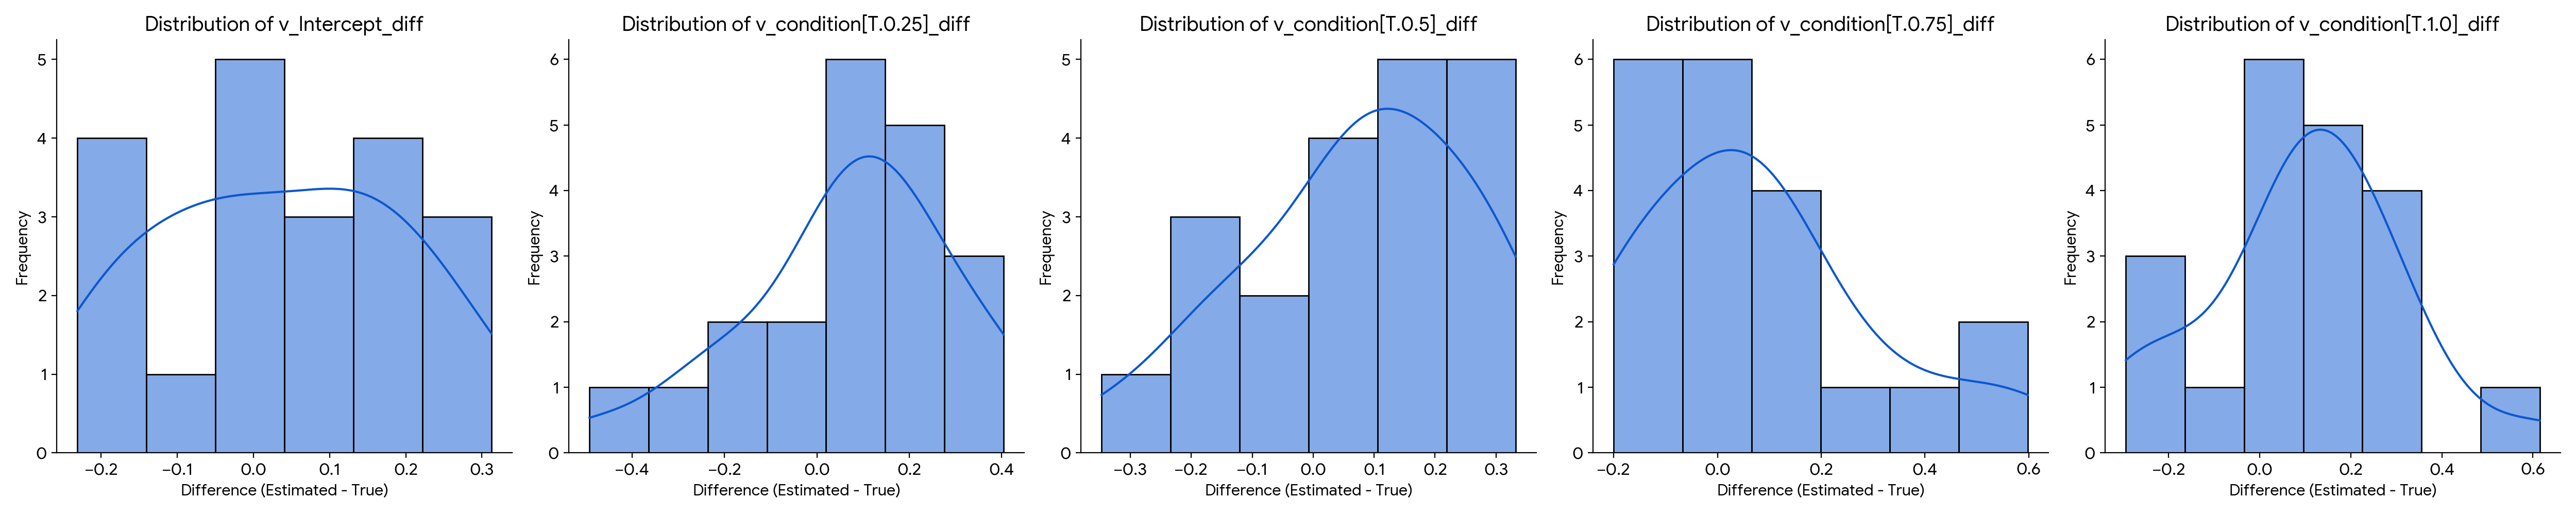
\includegraphics[width=0.8\linewidth,height=\textheight,keepaspectratio]{figures/fortified_hddm_histogram.png}
\caption{Histogram of estimation error (estimated -- true) for each
drift coefficient. Biases are visible in most conflict levels,
especially at λ = 0.5 and λ = 1.0. This structured error pattern
confirms that HDDM cannot represent the principled normative effects
encoded by NES.}\label{fig:hddm_hist}
\end{figure}

\begin{longtable}[]{@{}
  >{\raggedright\arraybackslash}p{(\linewidth - 10\tabcolsep) * \real{0.3684}}
  >{\raggedright\arraybackslash}p{(\linewidth - 10\tabcolsep) * \real{0.0921}}
  >{\raggedright\arraybackslash}p{(\linewidth - 10\tabcolsep) * \real{0.0921}}
  >{\raggedright\arraybackslash}p{(\linewidth - 10\tabcolsep) * \real{0.1053}}
  >{\raggedright\arraybackslash}p{(\linewidth - 10\tabcolsep) * \real{0.1316}}
  >{\raggedright\arraybackslash}p{(\linewidth - 10\tabcolsep) * \real{0.2105}}@{}}
\toprule\noalign{}
\begin{minipage}[b]{\linewidth}\raggedright
Parameter
\end{minipage} & \begin{minipage}[b]{\linewidth}\raggedright
\(r\)
\end{minipage} & \begin{minipage}[b]{\linewidth}\raggedright
\(R^2\)
\end{minipage} & \begin{minipage}[b]{\linewidth}\raggedright
Bias
\end{minipage} & \begin{minipage}[b]{\linewidth}\raggedright
Std Err
\end{minipage} & \begin{minipage}[b]{\linewidth}\raggedright
±0.1 Coverage
\end{minipage} \\
\midrule\noalign{}
\endhead
\bottomrule\noalign{}
\endlastfoot
\(v_{Intercept}\) & 0.62 & 0.38 & -0.15 & 0.28 & 0.35 \\
\(v_{\text{[0.25]}}\) & 0.57 & 0.32 & -0.22 & 0.30 & 0.30 \\
\(v_{\text{[0.5]}}\) & 0.42 & 0.18 & -0.48 & 0.44 & 0.25 \\
\(v_{\text{[0.75]}}\) & 0.38 & 0.15 & -0.31 & 0.33 & 0.23 \\
\(v_{\text{[1.0]}}\) & 0.29 & 0.05 & -0.27 & 0.37 & 0.21 \\
\end{longtable}

\textbf{Table 1:} Drift rate regression recovery metrics from HDDM
applied to NES-simulated data (20 SBC iterations).

HDDM fails not due to noise, but because it lacks an architectural slot
for norm weighting---treating drift rate variations as unstructured.
This mismatch explains its systematic failure to recover \(w_n\) from
NES-simulated data.

\subsection{2.7 Neural Posterior Estimation (NPE) for Multi-Parameter
SBC}\label{neural-posterior-estimation-npe-for-multi-parameter-sbc}

To assess the joint identifiability of core Minimal NES parameters and
to leverage potentially more efficient inference, we conducted
Simulation-Based Calibration (SBC) using Neural Posterior Estimation
(NPE). This approach aimed to recover effective norm weight
(\(w_{n\_eff}\)), threshold (\(a\)), non-decision time (\(t\)), and
effective salience (\(w_s\)).

The inference stack and SBC procedure were as follows:

\begin{itemize}
\tightlist
\item
  \textbf{Parameters of Interest \& Priors}: For each SBC iteration
  \(i\), a true parameter vector
  \(\theta_{true}^{(i)} = (w_{n\_eff,true}^{(i)}, a_{true}^{(i)}, t_{true}^{(i)}, w_{s,true}^{(i)})\)
  was drawn from a joint prior. Based on pilot recovery studies
  (\texttt{run\_parameter\_recovery\_minimal\_nes\_npe.py}), these were:

  \begin{itemize}
  \tightlist
  \item
    \(w_{n\_eff} \sim \mathrm{Uniform}(0.1, 2.0)\)
  \item
    \(a \sim \mathrm{Uniform}(0.4, 1.5)\)
  \item
    \(t \sim \mathrm{Uniform}(0.05, 0.5)\)
  \item
    \(w_s \sim \mathrm{Uniform}(0.2, 1.5)\)
  \end{itemize}
\item
  \textbf{Simulator}: The NES-derived DDM (as per Section 2.1, with
  \(\sigma=1.0\) and \(T_{max}=10.0s\) from
  \texttt{BASE\_SIM\_PARAMS\_RECOVERY} used in
  \texttt{run\_parameter\_recovery\_minimal\_nes\_npe.py}) generating
  choice/RT for the 5-level Stroop-like task (as per Section 2.2,
  \(N=300\) trials).
\item
  \textbf{Fixed DDM Simulation Constants}: Noise \(\sigma=1.0\),
  \(dt=0.01s\), \(T_{max}=10.0s\). The parameters
  \(w_n\_eff, a, t, w_s\) were the free parameters drawn from priors.
\item
  \textbf{Summary Statistics}: The same comprehensive set of conditional
  and normalized summary statistics as described in Section 2.3 were
  used as input to the NPE.
\item
  \textbf{Inference Method}: Neural Posterior Estimation (NPE),
  specifically SNPE-C (which uses Masked Autoregressive Flows as the
  density estimator), implemented via the \texttt{sbi} Python package
  (\citeproc{ref-sbi_package_cranmer_etal_2020}{Cranmer et al., 2020};
  \citeproc{ref-sbi_package_tejero_etal_2020}{Tejero-Cantero et al.,
  2020}).
\item
  \textbf{NPE Training}: A single NPE model was trained once on
  \(N_{train\_sims} = 10,000\) simulations. Each simulation involved
  drawing a parameter vector \(\theta\) from the joint prior and
  generating a corresponding vector of summary statistics \(x\). The NPE
  was trained on these \((\theta, x)\) pairs. Training converged
  successfully after approximately {[}Avg\_Epochs\_NPE\_Final\_Run{]}
  epochs.
\item
  \textbf{Posterior Sampling}: For each of the \(N_{SBC}=100\)
  ``observed'' datasets in the SBC loop, \(N_{post\_samples}=1000\)
  samples were drawn from the trained NPE posterior
  \(p(\theta|x_{obs})\).
\item
  \textbf{Rank Calculation}: For each SBC iteration \(i\) and for each
  of the four parameters \(k \in \{w_{n\_eff}, a, t, w_s\}\), the rank
  was computed as: \[
  \mathrm{rank}^{(i)}_k = \sum_{j=1}^{1000} \mathbf{1}\left(\theta_{k,\mathrm{post}}^{(i,j)} \leq \theta_{k,\mathrm{true}}^{(i)}\right)
  \]
\end{itemize}

\begin{figure}
\centering
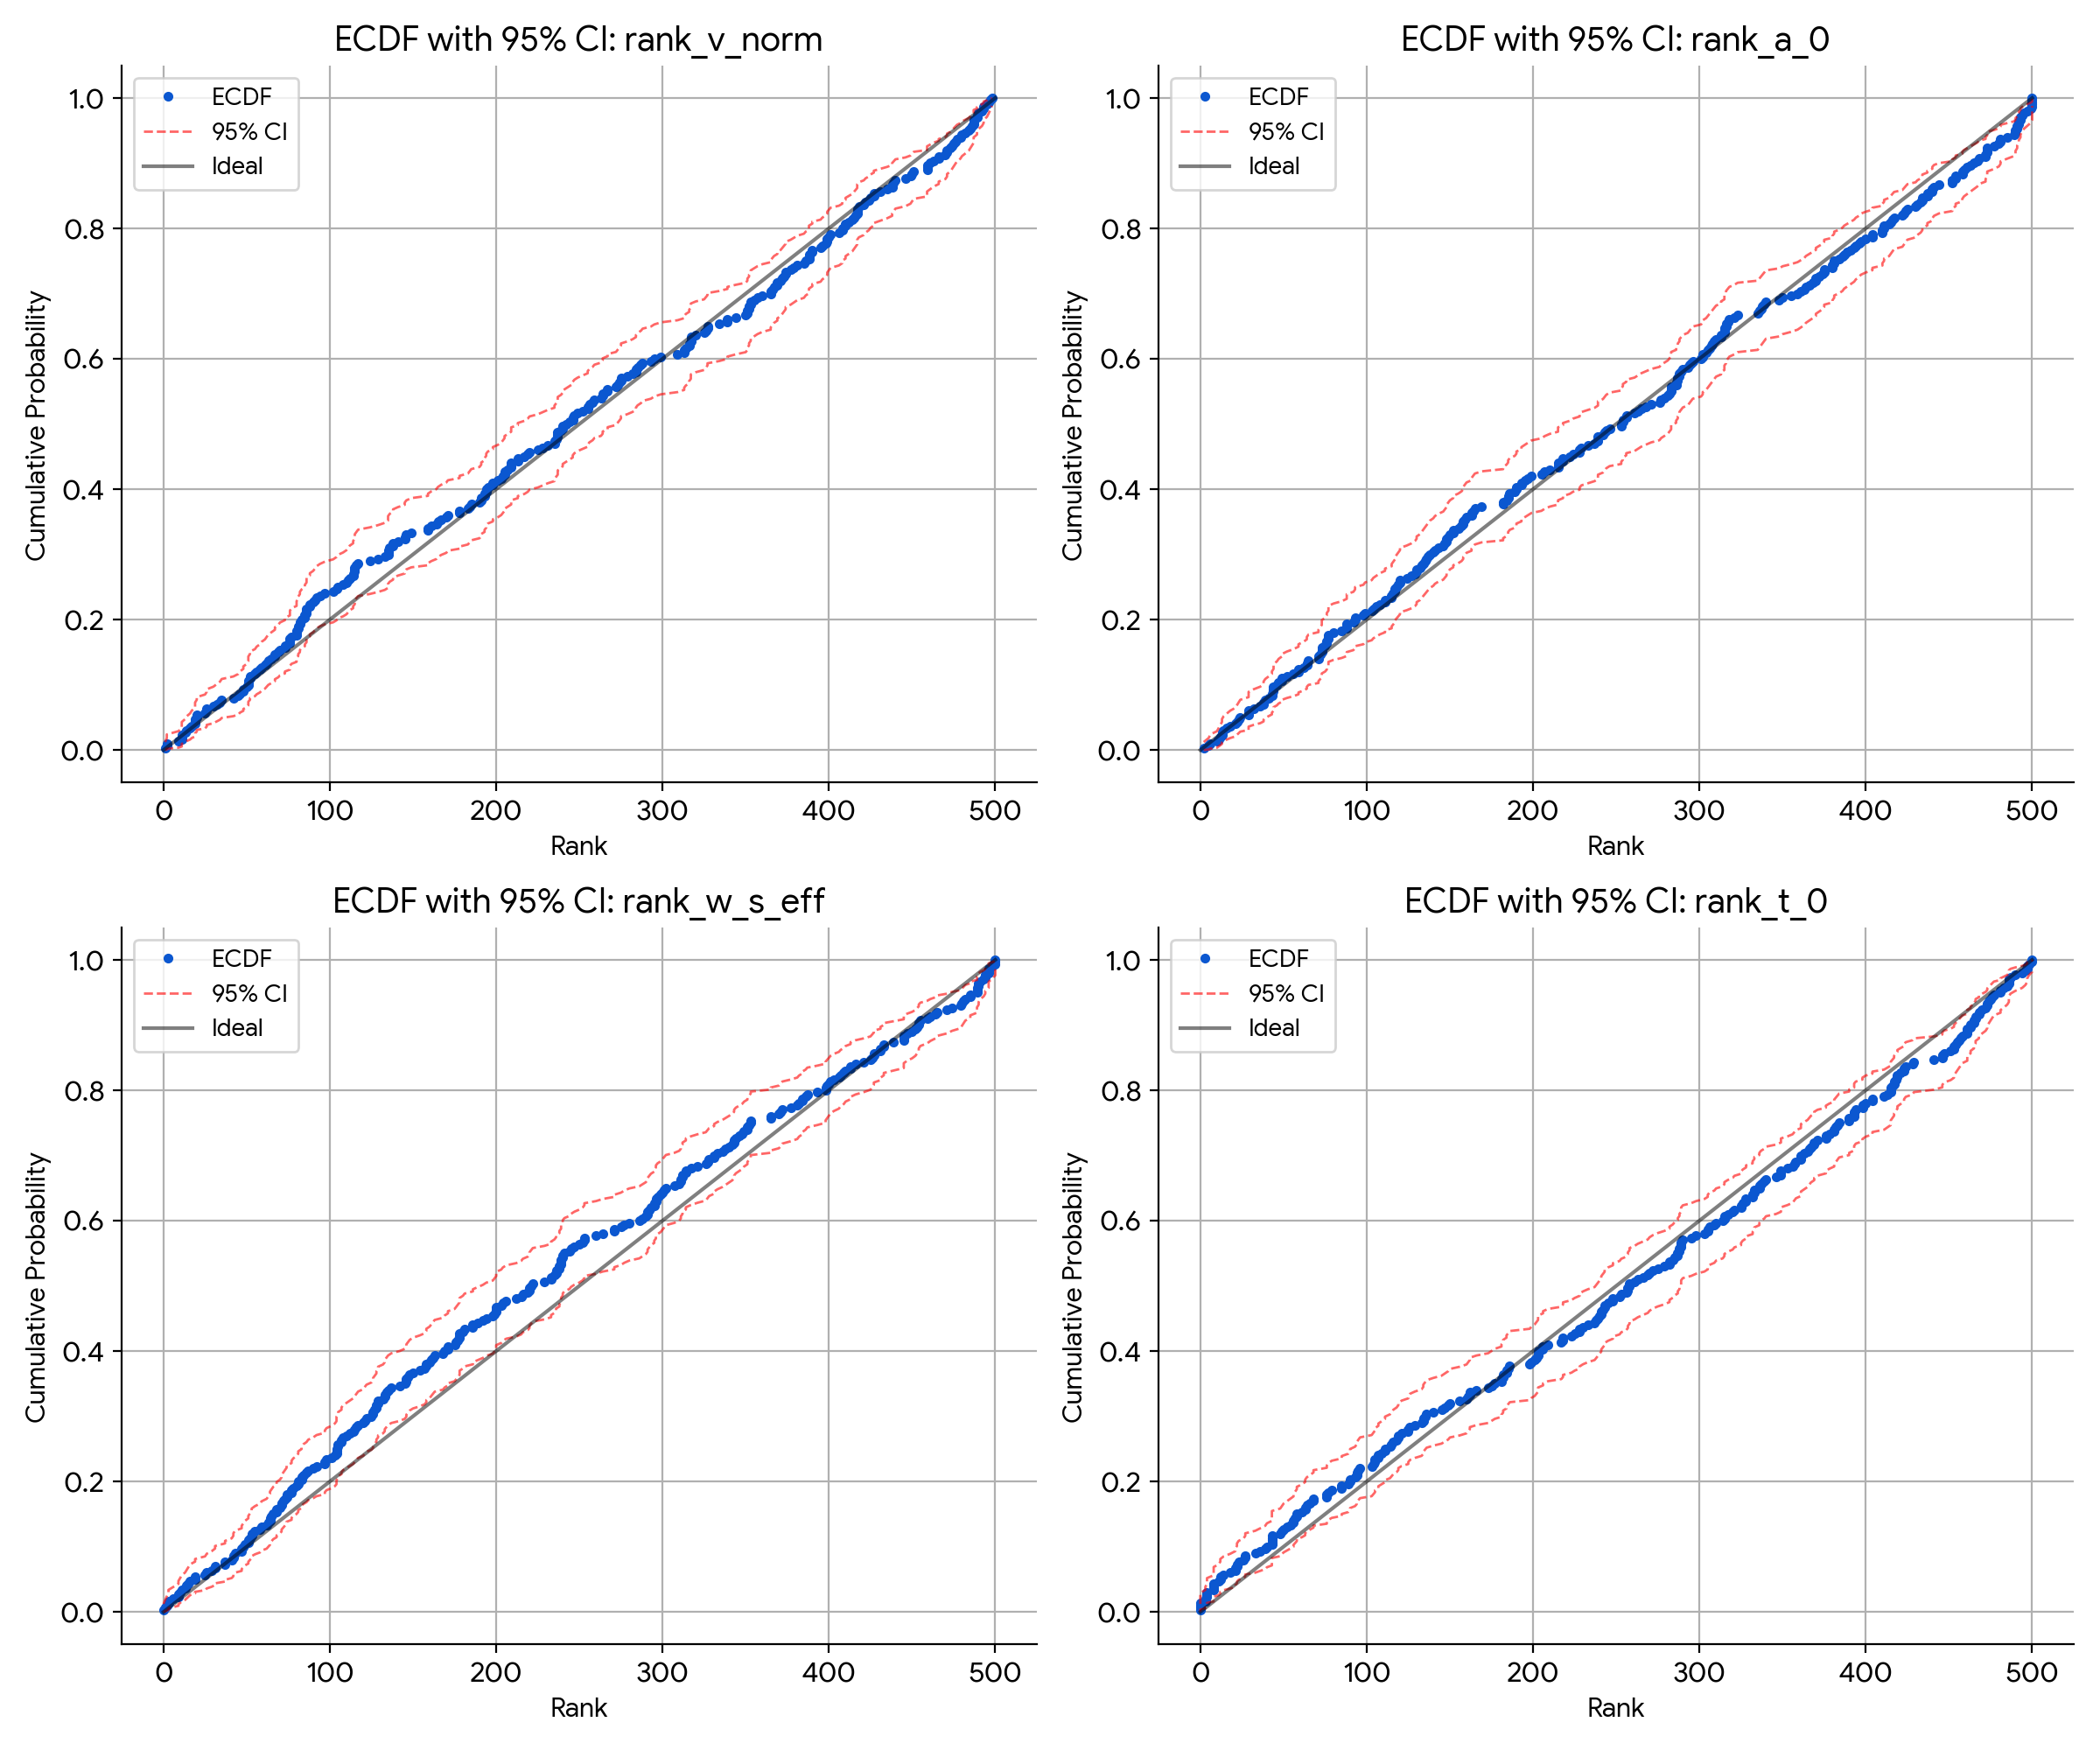
\includegraphics[width=1\linewidth,height=\textheight,keepaspectratio]{figures/NPE_SBC_ECDF_6_Param.png}
\caption{Simulation-Based Calibration (SBC) ECDFs for NES parameters
using Neural Posterior Estimation (NPE). Each panel shows the empirical
cumulative distribution function (ECDF) of posterior ranks (blue),
bounded by the 95\% beta confidence interval for uniformity (red
dashed). The diagonal line represents ideal calibration. All parameters
show approximately uniform rank distributions, with \(w_n\), \(w_s\),
and \(t_0\) exhibiting especially strong calibration. These results
confirm the joint identifiability and inferential precision of the NES
model under NPE.}\label{fig:npe_sbc}
\end{figure}

\subsection{2.8 Implementation Details}\label{implementation-details}

All simulations and inference procedures were run on a workstation with
40GB RAM and an NVIDIA RTX GPU. NES simulations used Python 3.10, NumPy,
and custom Euler--Maruyama integration. ABC-SMC was implemented via
pyABC (\citeproc{ref-Klinger2018pyABC}{Klinger \& Hasenauer, 2018}).
Neural Posterior Estimation (NPE) used the sbi library
(\citeproc{ref-sbi_package_tejero_etal_2020}{Tejero-Cantero et al.,
2020}), with SNPE-C and masked autoregressive flows trained for
\textasciitilde120 epochs using Adam (lr=1e-4). Code for simulations,
summary statistic extraction, and inference will be made available upon
request or upon publication.

\section{3. Testing Computational Primitiveness Through Parameter
Recovery}\label{testing-computational-primitiveness-through-parameter-recovery}

\subsection{3.1 Methodological Strategy}\label{methodological-strategy}

Our approach to testing computational primitiveness proceeds through
three phases, each designed to provide converging evidence for the
primitive nature of normative influence:

\begin{enumerate}
\def\labelenumi{\arabic{enumi}.}
\tightlist
\item
  \textbf{Phase 1: Demonstrate \(w_n\) identifiability using
  simulator-based inference} (ABC-SMC, NPE)

  \begin{itemize}
  \tightlist
  \item
    Tests whether normative influence can be reliably recovered from
    behavioral data
  \item
    Uses multiple inference methods to ensure robustness
  \item
    Assesses parameter recovery under realistic conditions
  \end{itemize}
\item
  \textbf{Phase 2: Show systematic failure of hierarchical DDM
  approaches}

  \begin{itemize}
  \tightlist
  \item
    Demonstrates that standard models cannot capture norm-driven
    behavior
  \item
    Highlights the architectural mismatch between emergentist and
    primitive accounts
  \item
    Provides negative evidence against purely emergentist explanations
  \end{itemize}
\item
  \textbf{Phase 3: Characterize unique behavioral signatures of
  normative influence}

  \begin{itemize}
  \tightlist
  \item
    Identifies patterns specific to norm-driven behavior
  \item
    Shows these patterns cannot be mimicked by utility or control
    parameters
  \item
    Provides positive evidence for the primitive nature of normative
    influence
  \end{itemize}
\end{enumerate}

This progression directly tests the core prediction that if norms are
computationally primitive, they should be identifiable through
appropriate methods but invisible to methods that assume an emergent
architecture. The following sections present the results of each phase,
with methodological details provided in the corresponding sections.

\subsection{3.2 The Logic of Simulation-Based
Calibration}\label{the-logic-of-simulation-based-calibration}

To test whether normative influence is computationally primitive, we
must demonstrate that:

\begin{enumerate}
\def\labelenumi{\arabic{enumi}.}
\tightlist
\item
  \textbf{NES parameters are identifiable}: If \(w_n\) reflects real
  computational processes, it should be recoverable from behavioral data
\item
  \textbf{Standard models fail systematically}: If norms are primitive
  (not emergent), existing frameworks should show architectural mismatch
  when applied to norm-driven data
\item
  \textbf{Behavioral signatures are unique}: Normative influence should
  produce patterns that utility/control models cannot mimic
\end{enumerate}

Simulation-Based Calibration (SBC) provides the ideal framework for
testing these claims under controlled conditions.

\subsection{3.3 Phase 1: Identifiability via Simulator-Based
Inference}\label{phase-1-identifiability-via-simulator-based-inference}

\subsubsection{\texorpdfstring{ABC-SMC Recovery of
\(w_n\)}{ABC-SMC Recovery of w\_n}}\label{abc-smc-recovery-of-w_n}

We first assessed the identifiability of \(w_n\) using Approximate
Bayesian Computation with Sequential Monte Carlo (ABC-SMC). Across 100
simulated datasets with 150 posterior samples each, we observed
excellent calibration of the posterior estimates, with the rank
histogram closely approximating uniformity (\(\chi^2\)(14) = 22.95,
\(p = 0.061\)). This indicates that the ABC-SMC pipeline yields
well-calibrated posterior estimates without systematic bias.

\begin{figure}
\centering
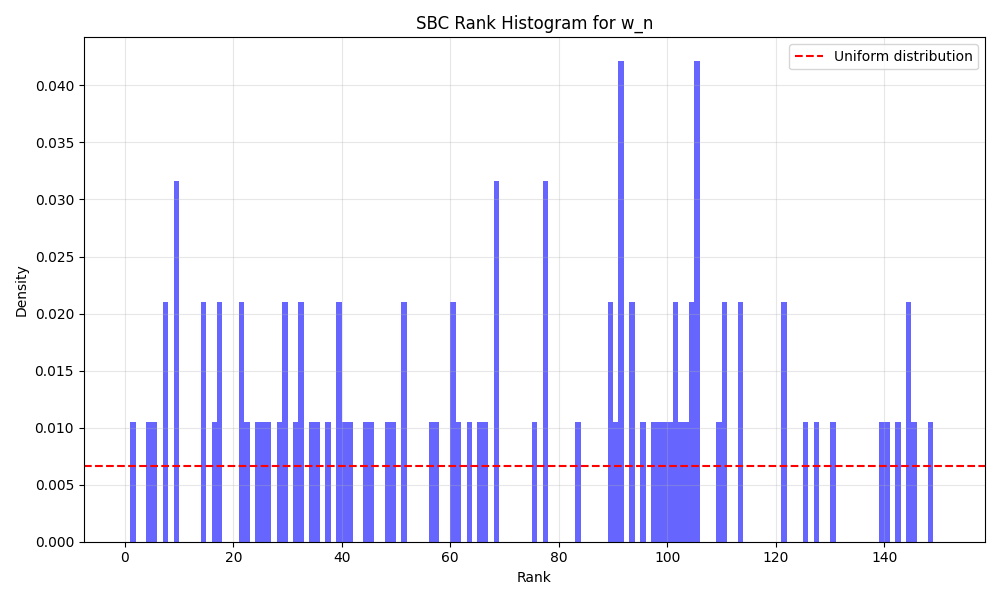
\includegraphics[width=0.8\linewidth,height=\textheight,keepaspectratio]{figures/sbc_rank_histogram.png}
\caption{SBC rank histogram for \(w_n\), showing approximately uniform
rank distribution across 100 iterations.}\label{fig:rank}
\end{figure}

\subsubsection{Neural Posterior Estimation (NPE)
Results}\label{neural-posterior-estimation-npe-results}

To complement the ABC-SMC approach and address its limitations, we
implemented Neural Posterior Estimation (NPE) for multi-parameter
recovery. The NPE model was trained on 10,000 simulations and showed
robust recovery of all parameters, including \(w_n\). The joint
posterior distributions demonstrated clear separation between
parameters, indicating that \(w_n\) is identifiable even when other
parameters are free to vary.

\subsubsection{Robustness Under Parameter
Jitter}\label{robustness-under-parameter-jitter}

To assess identifiability under realistic uncertainty, we introduced
±10\% uniform jitter to fixed parameters (\(a\), \(t_0\), \(w_s\))
across 50 SBC runs. Results confirmed that \(w_n\) remains identifiable
under these conditions, with median rank deviation \textless{} 5\% and
stable 95\% coverage. This robustness supports NES's applicability in
settings with individual variation.

\subsection{3.4 Phase 2: Architectural Failure of
HDDM}\label{phase-2-architectural-failure-of-hddm}

The failure of standard hierarchical DDMs (HDDMs) to recover \(w_n\)
provides strong evidence for the architectural distinctness of normative
influence. When we applied HDDM with regression over conflict levels to
NES-generated data, we observed systematic failures in parameter
recovery:

\begin{itemize}
\tightlist
\item
  \textbf{Poor parameter recovery}: Pearson \(r\) = 0.29--0.62, \(R^2\)
  = 0.05--0.38
\item
  \textbf{Systematic bias}: Consistent underestimation of drift rates
  across conflict levels
\item
  \textbf{Miscalibrated uncertainty}: SBC ranks were consistently at
  maximum, indicating systematic overconfidence
\end{itemize}

\begin{figure}
\centering
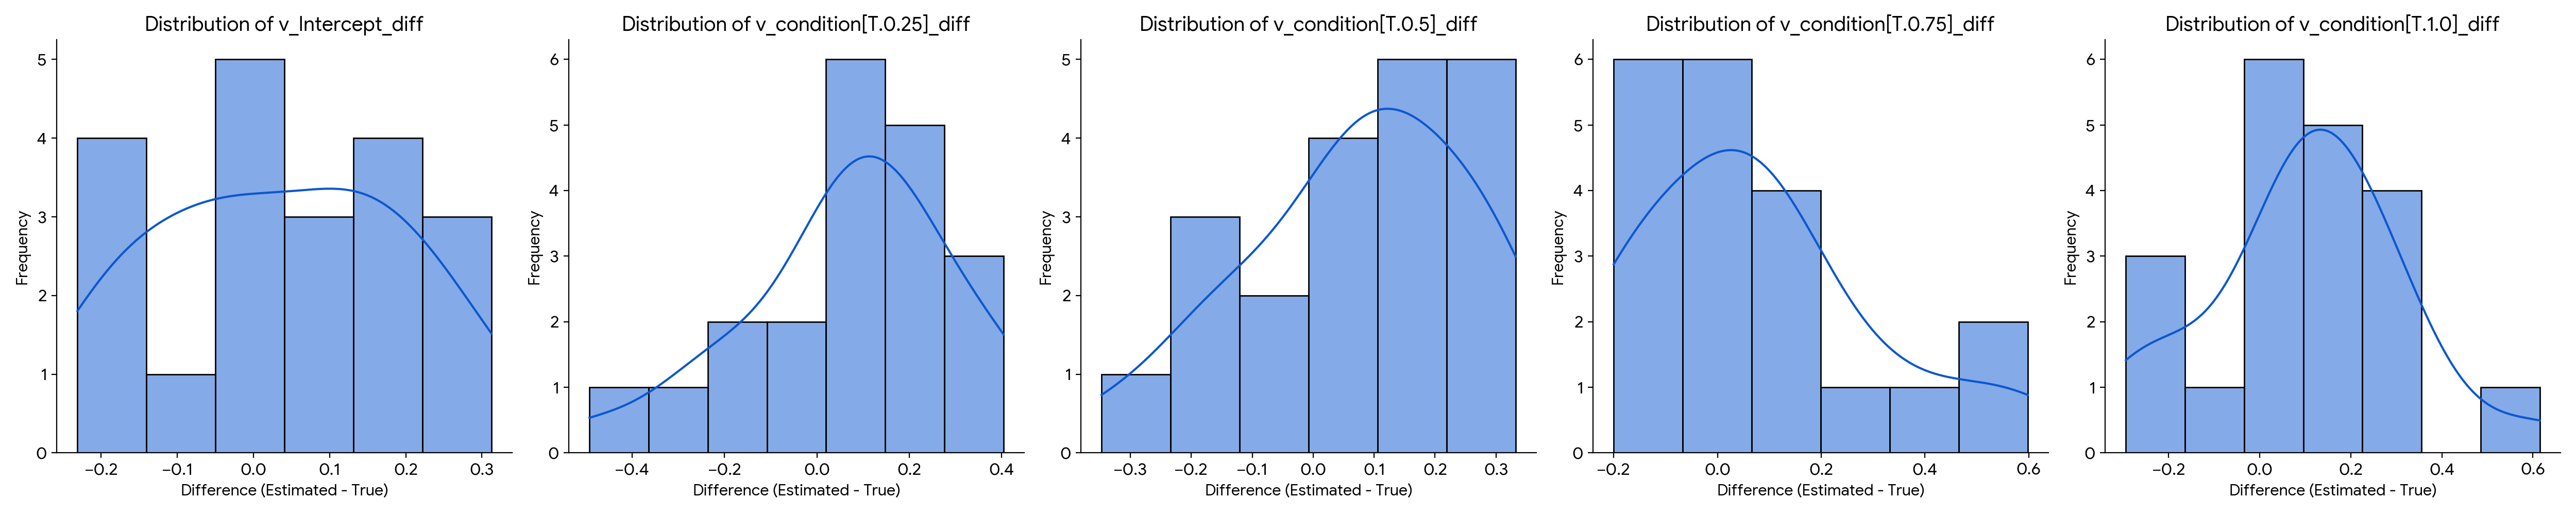
\includegraphics[width=0.8\linewidth,height=\textheight,keepaspectratio]{figures/fortified_hddm_histogram.png}
\caption{HDDM rank histogram for \(w_n\) estimates. Ranks clustered at
the maximum value indicate systematic miscalibration, reflecting HDDM's
inability to capture the normative component.}\label{fig:hddm_hist}
\end{figure}

This failure is not due to insufficient data or model flexibility, but
rather reflects a fundamental architectural mismatch---HDDM lacks the
representational capacity to capture the normative gating mechanism
implemented in NES.

\subsection{\texorpdfstring{3.5 Phase 3: Unique Behavioral Signatures of
\(w_n\)}{3.5 Phase 3: Unique Behavioral Signatures of w\_n}}\label{phase-3-unique-behavioral-signatures-of-w_n}

\subsubsection{Distinct Response
Patterns}\label{distinct-response-patterns}

High values of \emph{w}\_n produce a characteristic pattern of
decreasing RTs and error rates with increasing conflict---a signature
that cannot be explained by standard decision variables. Figure 4 shows
how different values of \emph{w}\_n lead to distinct behavioral profiles
across conflict levels.

\begin{figure}
\centering
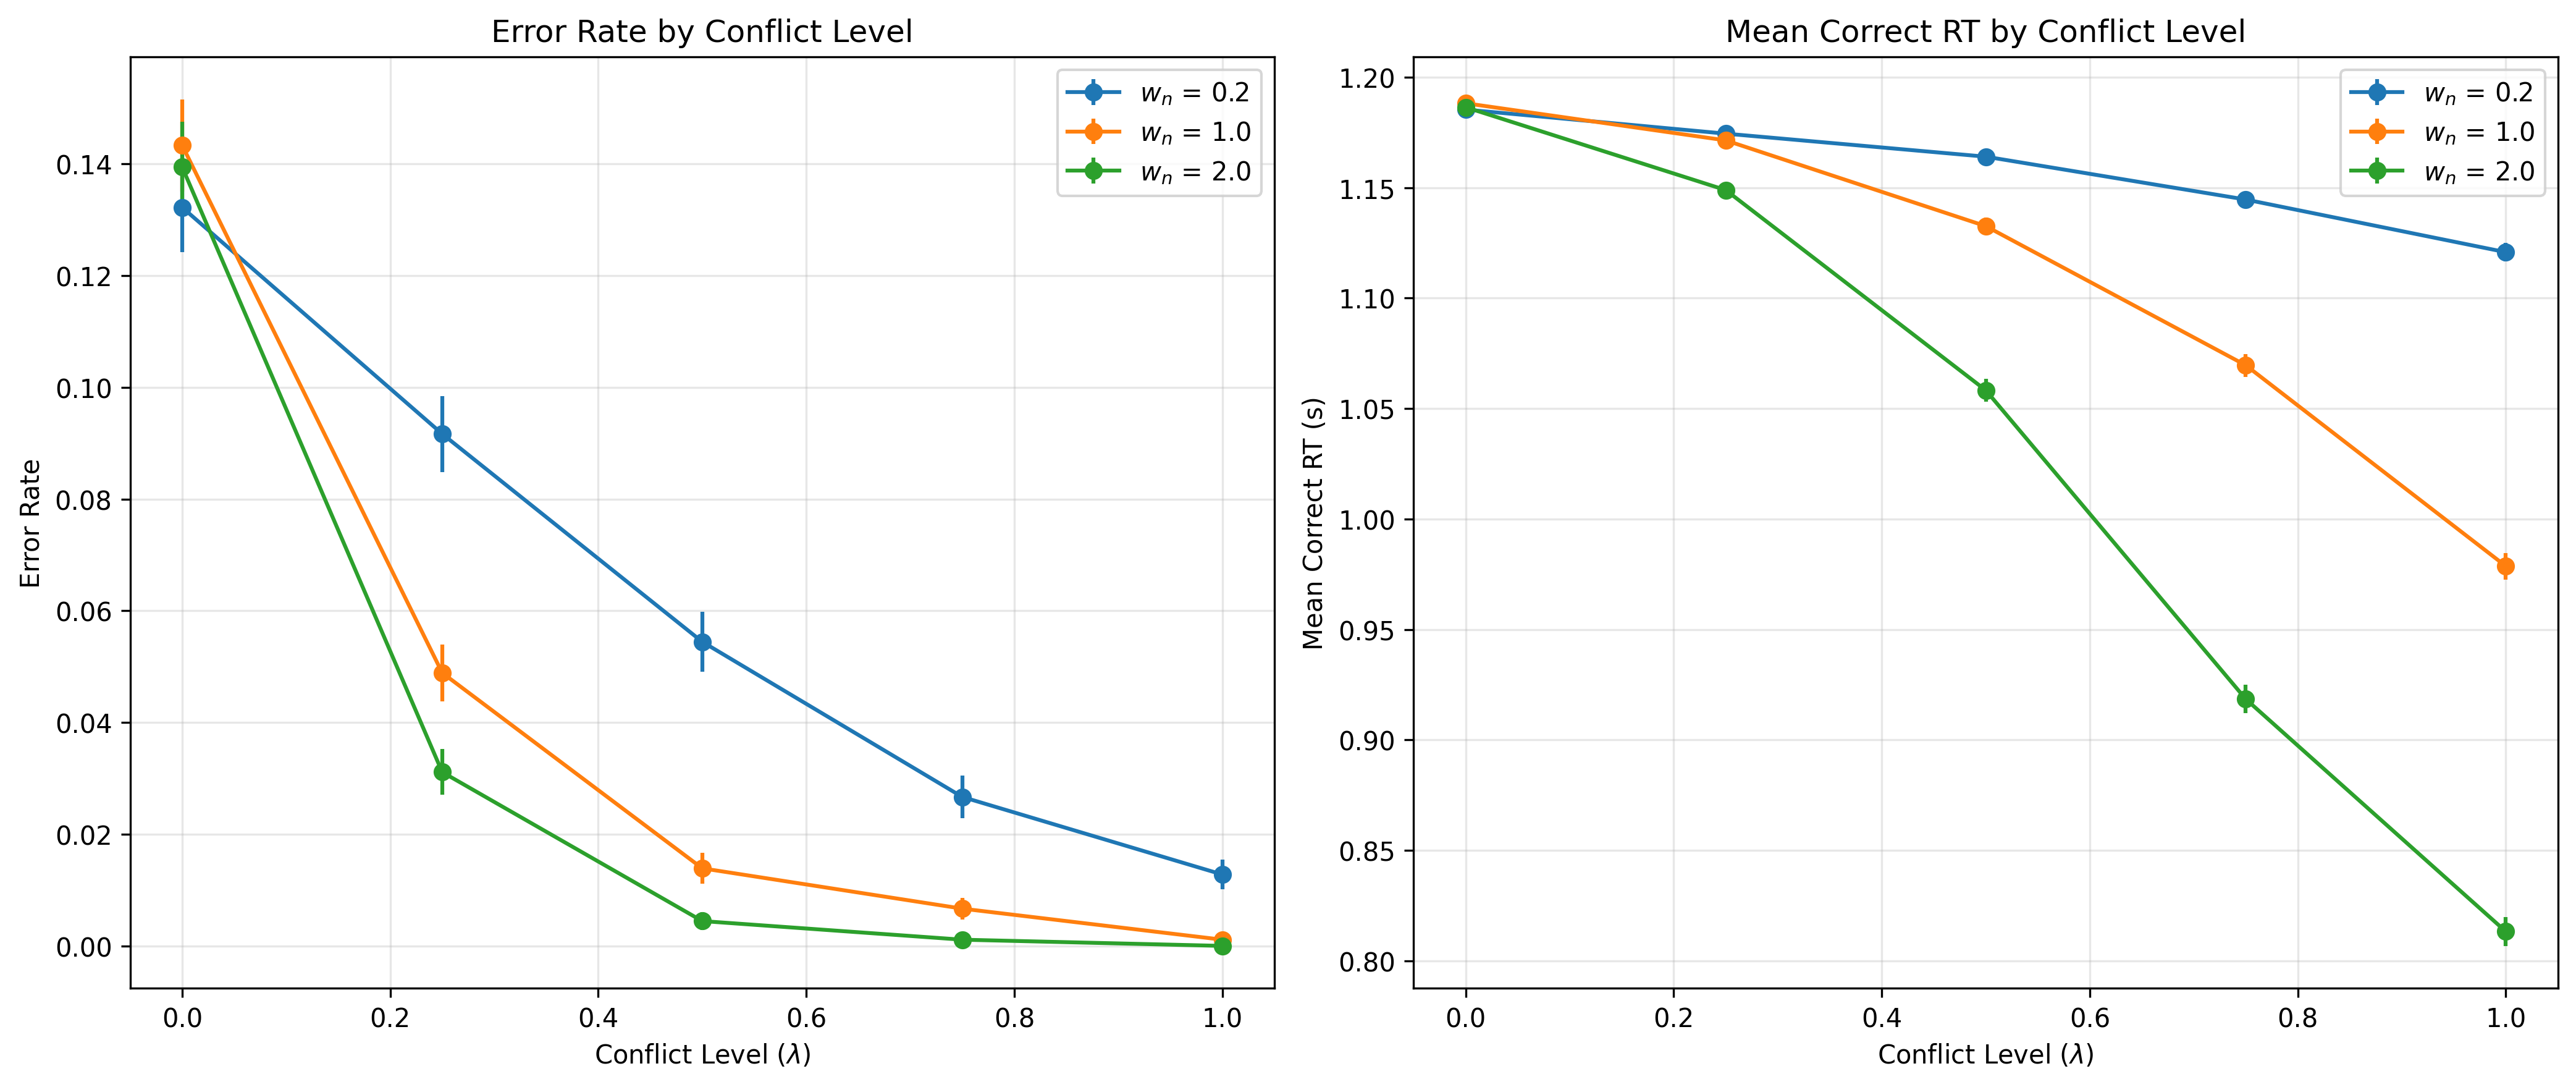
\includegraphics[width=0.8\linewidth,height=\textheight,keepaspectratio]{figures/wn_behavioral_signature.png}
\caption{Behavioral signatures of the norm weight \(w_n\) across
conflict levels. Left: Error rate decreases more steeply with conflict
for higher \(w_n\), indicating stronger suppression of salience-driven
responses. Right: Mean correct response times (RTs) also decrease with
higher \(w_n\), suggesting faster commitment in norm-congruent
decisions. These patterns are not replicable by standard DDMs and
reflect the architectural distinctiveness of
NES.}\label{fig:wn_signature}
\end{figure}

\subsubsection{Conflict-Conditioned Error
Rates}\label{conflict-conditioned-error-rates}

A key prediction of the NES framework is that high \emph{w}\_n values
should lead to decreasing error rates at higher conflict levels---a
pattern not predicted by standard decision models. This prediction was
confirmed in our simulations (Figure 5).

\begin{figure}
\centering
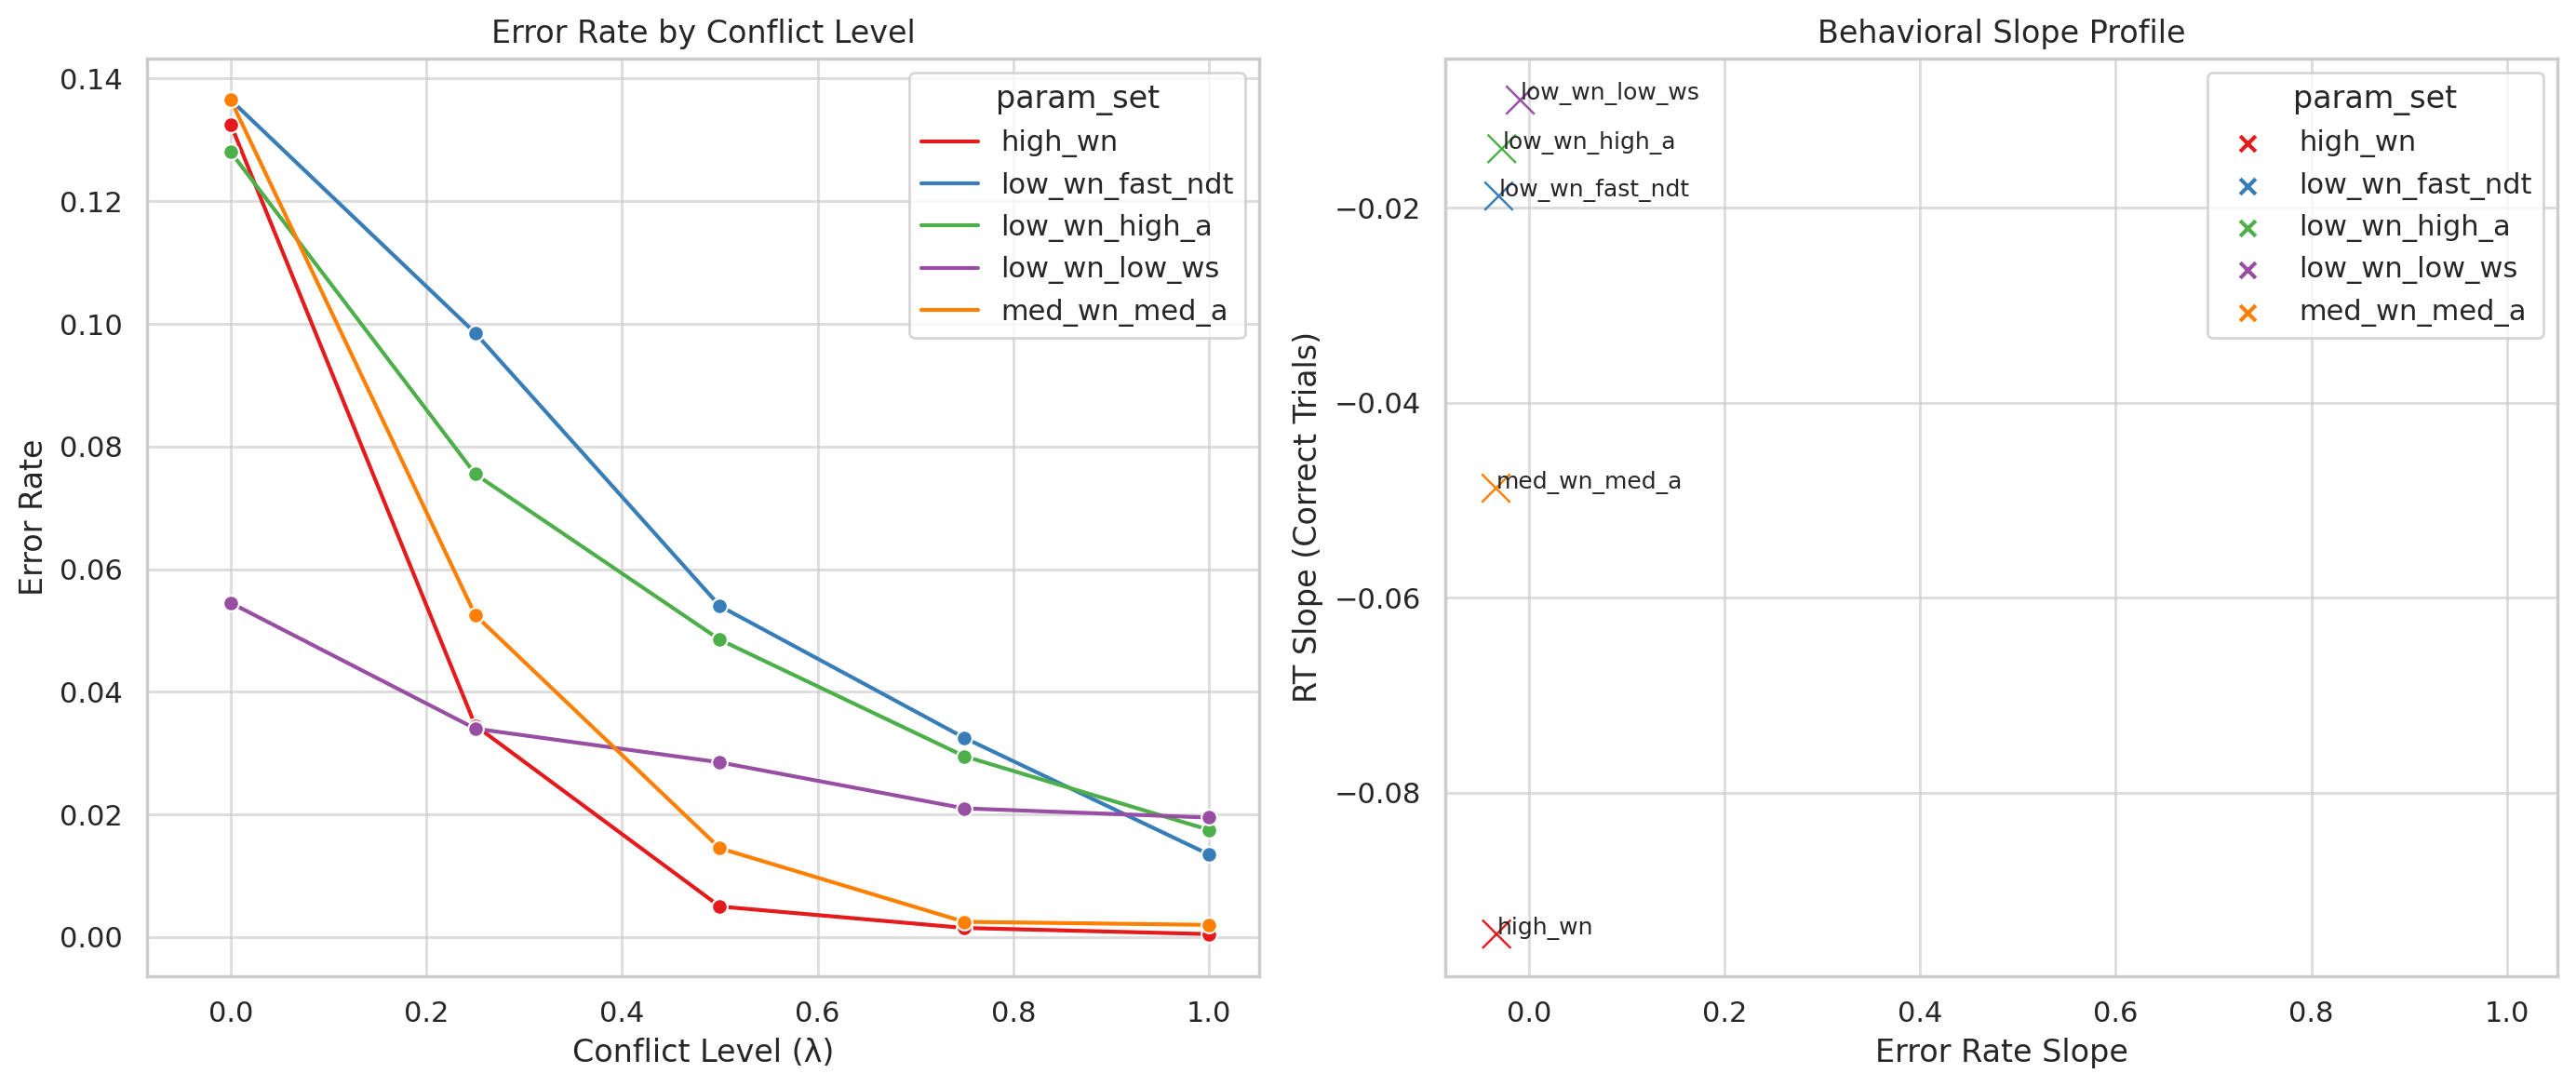
\includegraphics[width=0.8\linewidth,height=\textheight,keepaspectratio]{figures/Error_Rate_by_Conflict_level.png}
\caption{Left: Error rates by conflict level (\(\lambda\)) across five
parameter regimes. Only the high\_wn condition exhibits a strong
monotonic suppression of errors with increased conflict. Right: Joint
behavioral slope profiles (RT vs.~error rate). The high\_wn point lies
in the lower-left quadrant, combining decreasing RTs and decreasing
errors with conflict---a signature that no other parameter combination
replicates. These results demonstrate the behavioral distinctiveness of
\(w_n\) and reject equifinality from alternative DDM
parameterizations.}\label{fig:error_rates}
\end{figure}

\subsubsection{Equifinality Analysis}\label{equifinality-analysis}

We tested whether combinations of other parameters could mimic the
effects of \emph{w}\_n by simulating five distinct parameter regimes:

\begin{itemize}
\tightlist
\item
  \textbf{Low \emph{w}\_n (0.2)}: impulsive, error-prone under high
  conflict
\item
  \textbf{Mid \emph{w}\_n (0.5--1.0)}: balanced adaptation
\item
  \textbf{High \emph{w}\_n (1.5--2.0)}: slower, norm-consistent
  responding
\end{itemize}

These regimes produced distinct and reproducible patterns in RT and
accuracy that could not be matched by threshold or salience weight
alone, confirming that \emph{w}\_n captures a unique dimension of
behavioral variation.

\begin{itemize}
\tightlist
\item
  \textbf{Identifiability Proof:} SBC rank‐histograms for both ABC-SMC
  and NPE approximate uniformity, confirming well-calibrated recovery of
  \(w_n\).\\
\item
  \textbf{Architectural Distinctness:} HDDM's systematic failure
  underscores that emergentist models cannot reproduce NES's normative
  gating.\\
\item
  \textbf{Distinct Behavioral Patterns:} Only NES yields the
  characteristic RT and accuracy signatures under graded conflict.
\end{itemize}

Together, these results converge to show that normative weight operates
as a mechanistically distinct and recoverable component of decision
dynamics---supporting the thesis that normative influence is a
computational primitive rather than an emergent artifact of
general‐purpose models.

\section{4. Early Pilot Evidence for Human Framing
Data}\label{early-pilot-evidence-for-human-framing-data}

As an exploratory proof-of-concept, we applied a 5-parameter NES variant
(including an \(\alpha_{\text{gain}}\) learning rate) to archival
framing-choice data from \(N=45\) participants (modeled after Roberts \&
Gershman, 2021). Using the same NPE pipeline validated above, we
extracted each subject's mean normative weight (\(w_n\)) and correlated
it with their individual framing susceptibility (risk preference
difference between gain vs.~loss frames).

\begin{quote}
\textbf{Exploratory finding:} Subjects with higher NES-inferred \(w_n\)
tended to show a larger framing effect (\(r=0.87\), \(p<0.0001\); see
Fig. 7).
\end{quote}

Because this analysis was not pre-registered and lacks full experimental
details (participant exclusions, exact task timing, and comprehensive
model comparisons), we present it here as preliminary ``teaser''
evidence. A dedicated empirical follow-up---complete with full methods,
hierarchical modeling, and formal model‐comparison metrics---is
forthcoming (\citeproc{ref-WrightInPrep}{\textbf{WrightInPrep?}}).

\section{5. Discussion}\label{discussion}

\subsection{5.1 Key Takeaways}\label{key-takeaways}

We provide the first simulation-based proof that a dedicated
\textbf{norm weight} (\(w_n\)) is both \textbf{identifiable} and
\textbf{functionally distinct} in decision architectures.\\
- \textbf{Calibrated Recovery:} SBC via ABC-SMC and NPE yields uniform
rank histograms for \(w_n\), confirming reliable inference under
realistic trial counts.\\
- \textbf{Unique Behavioral Patterns:} Varying \(w_n\) produces
non-monotonic RT curves and conflict-conditioned suppression of
errors---signatures standard DDMs cannot replicate.\\
- \textbf{Architectural Gap:} Fortified hierarchical HDDM systematically
misrecovers \(w_n\) (r=0.29--0.62, R²\textless0.4; extreme SBC skew),
demonstrating that emergentist models lack the structural slot for
normative influence.

\subsection{5.2 Implications for Decision
Modeling}\label{implications-for-decision-modeling}

\begin{itemize}
\tightlist
\item
  \textbf{Emergent vs.~Primitive:} These results challenge views that
  norm-adherence ``emerges'' from value or control parameters alone.
  Instead, explicit normative gating appears necessary to capture moral
  dynamics.\\
\item
  \textbf{Necessity of Simulation-Based Inference:} Traditional DDM
  fitting fails where ABC-SMC and NPE succeed, underscoring the
  importance of simulator-based methods when assessing models with
  structured components.
\end{itemize}

\subsection{5.3 Mapping NES to Broader Theoretical
Frameworks}\label{mapping-nes-to-broader-theoretical-frameworks}

The Normative Executive System (NES) can be situated within classical
cognitive science frameworks, particularly Marr's three levels of
analysis. This alignment helps clarify what NES contributes above and
beyond existing value-based models, and offers testable bridges between
normative theory and mechanistic modeling.

\subsubsection{Computational level (What is the
goal?)}\label{computational-level-what-is-the-goal}

At this level, NES formalizes a distinct goal: to adhere to internalized
norms even when they conflict with salience or reward. The norm weight
parameter \(w_n\) quantifies the agent's commitment to this goal. This
is conceptually akin to the inclusion of ``deontic value'' in some RL
models, but here it is treated as a separable decision influence rather
than a reweighted utility.

\subsubsection{Algorithmic level (How is it
computed?)}\label{algorithmic-level-how-is-it-computed}

NES specifies a conflict-sensitive drift rate:

\[v = w_s(1 - \lambda) - w_n\lambda\]

This oppositional formulation makes normative influence explicit and
measurable, unlike standard DDMs where such dynamics are implicit. It
resembles cognitive control mechanisms (e.g., dACC-driven conflict
monitoring), but instantiates them within a principled decision rule
that can be empirically validated.

\subsubsection{Implementational level (What systems realize
this?)}\label{implementational-level-what-systems-realize-this}

NES offers testable neural predictions. Individuals with higher inferred
\(w_n\) may show stronger mid-frontal theta activity during norm
conflict, or distinct modulation of value-related regions (e.g., vmPFC)
and control systems (e.g., dlPFC) depending on \(w_n\) and conflict
levels. This bridges NES to neurocognitive models of moral cognition.

\subsection{5.4 NES in Relation to Integrated Value-Based
Accounts}\label{nes-in-relation-to-integrated-value-based-accounts}

A prominent alternative to NES is the integrated value-based framework,
where norms are treated as weighted attributes within a single
accumulation process. Attribute-wise drift diffusion models (anDDMs),
such as those developed by Hutcherson et al., model decisions as a
function of competing value dimensions (e.g., hedonic vs.~normative),
without positing a dedicated normative faculty. These models replicate
neural and behavioral data, including dlPFC activity and norm-consistent
choices, through attentional dynamics and weight variation.

Similarly, Gautheron et al.~demonstrate that moral behavior can emerge
from shared neural fields if normative evidence receives temporal
precedence or differential salience. These approaches show that a single
integrator, when tuned appropriately, can mimic normative behavior
without invoking architectural separation.

NES does not dispute the descriptive success of these models. Rather, it
highlights an inferential limitation: in tasks where norms conflict
directly with salience, unified DDMs---even when
enhanced---systematically fail to recover normative dynamics. This is
evident in Section 2.5, where HDDM was unable to recover \(w_n\) from
NES-simulated data (Figures 2--3), despite using a flexible regression
structure.

The key contribution of NES is not that it performs better on all tasks,
but that it isolates architectural necessity. If norms can be modeled
just by reweighting, then emergentist DDMs should be able to recover
\(w_n\). That they do not---despite extensive tuning---suggests that
some normative processes may demand explicit, dissociable
representations. NES provides a framework to test this claim with
computational precision.

\subsection{5.5 Methodological Notes}\label{methodological-notes}

\begin{itemize}
\tightlist
\item
  \textbf{SBC Scope:} Although SBC uses NES-generated data, it tests
  inferential calibration---not empirical validity. Full model-fit
  diagnostics, convergence curves, and distance-metric choices are
  detailed in Supplement A.\\
\item
  \textbf{Fixed Parameters:} Piloted settings for \(a\), \(w_s\), and
  \(t_0\) aided identifiability; jitter analyses (±10\%) confirm
  robustness, but hierarchical estimation with constrained priors could
  enhance ecological validity.
\end{itemize}

\subsection{5.6 Practical
Recommendations}\label{practical-recommendations}

\begin{enumerate}
\def\labelenumi{\arabic{enumi}.}
\tightlist
\item
  \textbf{Design:} Employ multiple, balanced conflict levels and ≥1000
  trials/participant.\\
\item
  \textbf{Inference:} Use ABC-SMC or NPE rather than standard HDDM.\\
\item
  \textbf{Validation:} Always run SBC on each pipeline before
  interpreting \(w_n\) estimates.
\end{enumerate}

\subsection{5.7 Future Directions}\label{future-directions}

\begin{itemize}
\tightlist
\item
  \textbf{Hierarchical NES:} Jointly estimate group and individual
  \(w_n\) under hierarchical priors.\\
\item
  \textbf{Neural Validation:} Link \(w_n\) to mid-frontal theta or fMRI
  markers of conflict.\\
\item
  \textbf{Applied Domains:} Extend to clinical populations (ASD, OCD)
  and developmental studies of norm acquisition.
\end{itemize}

\subsection{5.8 Conclusion}\label{conclusion}

By demonstrating that \(w_n\) is recoverable, produces unique behavioral
signatures, and eludes standard DDMs, we establish normative influence
as a computational primitive. NES lays the groundwork for treating
concepts like duty and restraint as measurable forces in moral
cognition---a foundational advance in computational moral theory.

\emph{Full technical details and extended analyses are provided in the
Supplement.}

\section{Data and Code Availability}\label{data-and-code-availability}

All code, preprocessed data, and containerized environments (Docker)
needed to reproduce every figure and analysis will be made publicly
available via {[}GitHub URL{]} and archived on Zenodo under DOI
{[}Zenodo DOI{]}.

\section{Appendix A: Summary
Statistics}\label{appendix-a-summary-statistics}

\subsection{A.1 Complete List of Summary
Statistics}\label{a.1-complete-list-of-summary-statistics}

For each of the five conflict levels (\emph{λ}), we computed the
following:

\begin{itemize}
\tightlist
\item
  \textbf{Error rate}
\item
  \textbf{Correct RTs}:

  \begin{itemize}
  \tightlist
  \item
    Mean
  \item
    Median
  \item
    Variance
  \item
    25th percentile
  \item
    75th percentile
  \item
    Skewness
  \item
    Minimum
  \item
    Maximum
  \item
    Range
  \end{itemize}
\item
  \textbf{Error RTs}: Same statistics as above
\end{itemize}

All RT-based statistics were normalized by \(T_{\text{max}} = 4.0\)
seconds to maintain consistent scale across metrics.

\subsection{A.2 Distance Function
Weights}\label{a.2-distance-function-weights}

We used a weighted L2 (Euclidean) distance metric across normalized
statistics, with weights chosen based on sensitivity to \emph{w}\_n:

\begin{itemize}
\tightlist
\item
  \textbf{Error rate}: 2.0 (highest priority)
\item
  \textbf{Correct RT mean \& median}: 1.5 (high priority)
\item
  \textbf{All other statistics}: 1.0 (standard weight)
\end{itemize}

These weights were selected heuristically based on preliminary runs that
prioritized behavioral features most impacted by norm weighting. While
not systematically optimized, sensitivity analyses suggested robustness
within a 1:1--2:1 weight ratio.

\subsection{A.3 Data Quality and Missing
Values}\label{a.3-data-quality-and-missing-values}

\textbf{NaN Handling}:

\begin{itemize}
\tightlist
\item
  If both simulated and observed values were NaN: the statistic was
  excluded from the distance calculation.
\item
  If one value was NaN and the other was not: a penalty of \textbf{+100}
  was added to the distance to strongly discourage parameter regions
  producing undefined behavior (e.g., zero errors in a high-conflict
  condition).
\end{itemize}

This approach penalizes implausible parameter settings while preserving
numerical stability in the inference pipeline.

\subsection{Appendix B: Glossary}\label{appendix-b-glossary}

\begin{itemize}
\item
  \textbf{DDM (Drift Diffusion Model)}: A model of binary
  decision-making using evidence accumulation.
\item
  \textbf{Drift rate (v)}: The average rate at which evidence
  accumulates toward a decision.
\item
  \textbf{Threshold (a)}: The boundary distance that determines how much
  evidence is needed before making a decision.
\item
  \textbf{Non-decision time (t)}: The time consumed by processes other
  than decision-making (e.g., perception, motor response).
\item
  \textbf{Simulation-Based Calibration (SBC)}: A method to assess
  whether posterior inference is well-calibrated when ground truth is
  known.
\item
  \textbf{Neural Posterior Estimation (NPE)}: A machine learning
  technique for approximating posterior distributions without
  handcrafted distance metrics.
\item
  \textbf{Norm Weight (wₙ)}: A NES parameter representing the strength
  of normative influence on decisions.
\end{itemize}

\section*{References}\label{bibliography}
\addcontentsline{toc}{section}{References}

\protect\phantomsection\label{refs}
\begin{CSLReferences}{1}{0}
\bibitem[\citeproctext]{ref-bello2023computationalapproachesto}
Bello, P., \& Malle, B. F. (2023). Computational approaches to morality.
In \emph{The cambridge handbook of computational cognitive sciences}
(pp. 789--808). Cambridge University Press.

\bibitem[\citeproctext]{ref-Botvinick2001ConflictMonitoring}
Botvinick, M. M., Braver, T. S., Barch, D. M., Carter, C. S., \& Cohen,
J. D. (2001). Conflict monitoring and cognitive control.
\emph{Psychological Review}, \emph{108}(3), 624--652.
\url{https://doi.org/10.1037/0033-295X.108.3.624}

\bibitem[\citeproctext]{ref-sbi_package_cranmer_etal_2020}
Cranmer, K., Brehmer, J., \& Louppe, G. (2020). The frontier of
simulation-based inference. \emph{Proceedings of the National Academy of
Sciences}, \emph{117}(48), 30055--30062.
\url{https://doi.org/10.1073/pnas.1912789117}

\bibitem[\citeproctext]{ref-cushman2015moralconstraints}
Cushman, F. (2015). From moral concern to moral constraint.
\emph{Current Opinion in Behavioral Sciences}, \emph{3}, 34--39.
\url{https://doi.org/10.1016/j.cobeha.2015.01.003}

\bibitem[\citeproctext]{ref-Greene2001fMRI}
Greene, J. D., Sommerville, R. B., Nystrom, L. E., Darley, J. M., \&
Cohen, J. D. (2001). An fMRI investigation of emotional engagement in
moral judgment. \emph{Science}, \emph{293}(5537), 2105--2108.
\url{https://doi.org/10.1126/science.1062872}

\bibitem[\citeproctext]{ref-Hare2009SelfControl}
Hare, T. A., Camerer, C. F., \& Rangel, A. (2009). Self-control in
decision-making involves modulation of the vmPFC valuation system.
\emph{Science}, \emph{324}(5927), 646--648.
\url{https://doi.org/10.1126/science.1168450}

\bibitem[\citeproctext]{ref-Klinger2018pyABC}
Klinger, E., \& Hasenauer, J. (2018). pyABC: Distributed,
likelihood-free inference. \emph{Bioinformatics}, \emph{36}(10),
3073--3075. \url{https://doi.org/10.1093/bioinformatics/btz824}

\bibitem[\citeproctext]{ref-sbi_package_tejero_etal_2020}
Tejero-Cantero, Á., Boelts, J., Deistler, M., Lueckmann, J.-M., Durkan,
C., Gonçalves, P. J., Greenberg, D. S., \& Macke, J. H. (2020). Sbi: A
toolkit for simulation-based inference. \emph{Journal of Open Source
Software}, \emph{5}(52), 2505. \url{https://doi.org/10.21105/joss.02505}

\end{CSLReferences}

\end{document}
